\chapter{Contexte}\label{chap:contexte}

    Mon stage de fin d'études s'est déroulé au sein d'IMT Atlantique, sur le
    campus de Rennes. Ce chapitre détaille le contexte global de mon stage en
    suivant un plan en entonnoir, allant de l'organisation générale d'IMT
    Atlantique jusqu'à mes missions spécifiques au sein du projet ANR
    \textit{Towards Public Blockchain for Self-Sovereign Identities}~\cite{anr},
    dans le cadre duquel mon stage s'est déroulé.

\section{IMT Atlantique}\label{sec:imt_atlantique} 

    % Imt atlantique
    IMT Atlantique, de l'Institut Mines-Télécom, est une école d'ingénieurs
    française issue de la fusion, en janvier 2017, de l'École nationale
    supérieure des mines de Nantes et de Télécom Bretagne. L'école possède trois
    campus situés à Brest, Nantes et Rennes. Elle propose des formations
    d'ingénieurs pluridisciplinaires couvrant les domaines des sciences, des
    technologies de l'information, de la communication, et des mathématiques. En
    termes de recherche, IMT Atlantique est structurée en douze départements
    d'enseignement et de recherche, regroupant des enseignants-chercheurs
    affiliés à différentes Unités Mixtes de Recherche (UMR) dont le GEPEA
    \footnote{\href{https://www.gepea.fr}{https://www.gepea.fr}}, l'IRISA
    \footnote{ \href{https://www.irisa.fr}{https://www.irisa.fr}}, et le
    Lab-STICC \footnote{\href{https://labsticc.fr}{https://labsticc.fr}}. Parmi
    ces douze départements, on trouve le département de Systèmes Réseaux,
    Cybersécurité et Droit du numérique (SRCD) sur le campus de Rennes, dans
    lequel j'ai effectué mon stage.

    % Le département SRCD
    Le département SRCD est composé à ce jour de 27 enseignants-chercheurs
    permanents, plus de 10 post-doctorants et ingénieurs contractuels, 31
    doctorants et 4 stagiaires. Les activités de recherche du département sont
    articulées autour de trois grands axes: les systèmes réseaux, la
    cybersécurité, et le droit du numérique. Les enseignants-chercheurs du
    département SRCD participent, avec des collègues d'autres institutions
    (\emph{e.g.,} Université de Rennes), à 6 équipes de l'IRISA, dont l'équipe
    SOTERN
    \footnote{\href{https://www.irisa.fr/sotern/}{https://www.irisa.fr/sotern/}}
    qui a accueilli mon stage.

    % Équipe SOTERN
    L'équipe SOTERN, pour Self-prOtecting The futurE inteRNet, s'articule autour
    du deuxième pilier de recherche du département SRCD~: la cybersécurité.
    C'est une équipe qui a été créée en début d'année 2023 et qui est dirigée
    par Guillaume Doyen, professeur à IMT Atlantique. L'équipe compte
    aujourd'hui 9 membres permanents, 1 post-doctorant, 6 doctorants et 5
    stagiaires. Les recherches de cette équipe se concentrent sur la conception,
    le développement et la validation de méthodes et d'outils pour
    l'auto-protection de l'Internet futur. Le projet ANR à l'origine de mon stage
    s'inscrit dans le cadre des recherches menées par l'équipe SOTERN.


\section{Projet BC4SSI}\label{sec:bc4ssi} 

    Mon tuteur, Romaric Ludinard, est le coordinateur du projet ANR intitulé
    BC4SSI~\cite{anr} (\textit{Towards Public Blockchain for Self-Sovereign
    Identities}). Ce projet s'inscrit dans l'axe E.3 /CES 25 de l'ANR, qui se
    concentre sur les verrous scientifiques relatifs aux réseaux de
    communication, architectures de réseau, et technologies logicielles, avec
    une attention particulière aux technologies Blockchain, et aux systèmes
    distribués. Plus spécifiquement, le projet BC4SSI à pour objectif de chercher
    des solutions aux verrous scientifiques et technologiques en lien avec les
    systèmes Blockchain, tels que décrit dans le rapport d'avril 2021 de la
    Direction Générale des Entreprises détaillant les principaux défis et enjeux
    de tels systèmes en France~\cite{dge}. Mon travail s'est concentré sur le
    verrou numéro 2, qui concerne la compression de structures de données de
    type Blockchain. J'ai rejoint le projet en février 2024, c'est-à-dire 12
    mois après le début de celui-ci. Quand je suis arrivé, un article de recherche
    était en cours de rédaction, et j'ai contribué à l'écriture des sections
    restantes.


\section{Mes missions}\label{sec:mes_missions}

    Les deux à trois premiers mois de mon stage au sein de l'équipe SOTERN ont
    été consacrés à la réalisation d'un état de l'art. Cette phase initiale
    était essentielle pour plusieurs raisons. La première était de me
    familiariser avec le sujet complexe de la Blockchain : cette période
    d'analyse des publications m'a aidé à identifier les solutions actuellement
    explorées dans le domaine. La seconde raison était de commencer à
    appréhender les outils et les concepts utilisés dans notre article. La fin
    de cette phase documentaire a donc été un mélange entre la lecture de la
    littérature et la reconstruction des preuves mathématiques détaillées dans
    les articles les plus proches de notre sujet, afin d'acquérir une
    compréhension fine des outils dont j'allais avoir besoin pour la seconde
    partie de mon stage.

    La seconde partie de mon stage a été consacrée à la rédaction de l'article
    de recherche. L'objectif était de proposer une solution pour compresser les
    structures de données de type Blockchain. Une telle solution existait déjà,
    mais elle fonctionnait dans un cadre très particulier : le cas où la
    population du système reste constante. Nous avons donc cherché à généraliser
    cette solution pour qu'elle fonctionne dans le cadre plus large d'un système
    à la population variable. J'ai donc participé à la fabrication de plusieurs
    modèles pour décrire notre problème et aux travaux mathématiques nécessaires
    pour démontrer la validité de nos propositions. J'ai également créé un
    programme de calcul qui implémente nos modèles afin d'obtenir des résultats
    numériques.


\section{Environnement de travail}\label{sec:contexte_de_travail}

    Au quotidien, j'ai travaillé avec les 4 personnes qui constituaient le pôle
    Blockchain de l'équipe SOTERN. Romaric Ludinard, mon tuteur, enseignant
    chercheur à IMT Atlantique, Loïc Miller, post-doctorant à IMT Atlantique
    également, Dorian Pacaud, Stagiaire qui a commencé 1 mois après moi, et
    Emmanuelle Anceaume, Directrice de Recherche au CNRS, membre de l'équipe
    PIRAT\textbackslash\textquotesingle);
    \footnote{\href{https://www.inria.fr/pirat}{https://www.inria.fr/pirat}} de
    l'IRISA.

    \vspace{0.4cm}
    \begin{figure}[ht]
        \centering
        \sbox0{\begin{tabular}{rl}
		\tikz{\node[fill=red!40, draw=black, inner sep=1ex]{};} & IMT Atlantique\\
		\tikz{\node[fill=green!40, draw=black, inner sep=1ex]{};} & SRCD\\
		\tikz{\node[fill=blue!40, draw=black, inner sep=1ex]{};} & SOTERN\\
		\tikz{\node[shape=circle, dotted, line width=2pt, draw=black, inner sep=0.5ex]{};} & BC4SSI
	\end{tabular}}

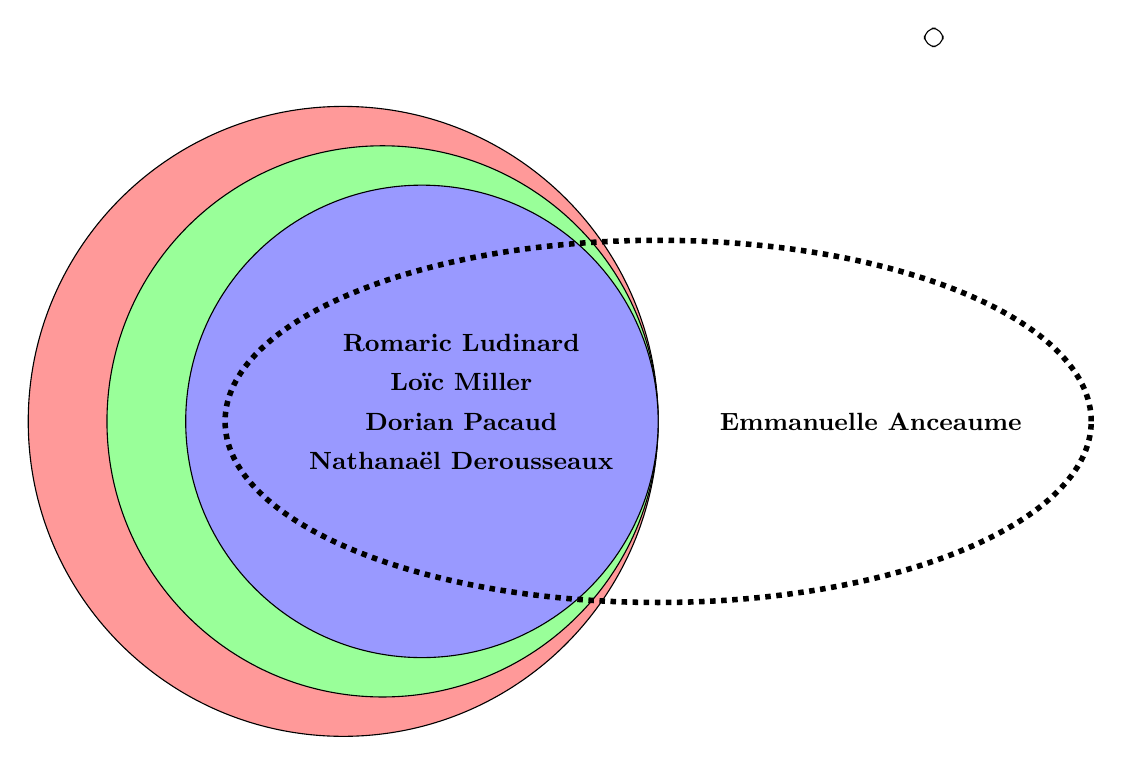
\begin{tikzpicture}[scale=1]
		\begin{scope}[shift={(3cm,-5cm)}, fill opacity=1]
				
				% Ellipses
				\draw[fill=red!40, draw=black] (0,0) circle (4);
				\draw[fill=green!40, draw=black] (0.5,0) circle (3.5);
				\draw[fill=blue!40, draw=black] (1,0) circle (3);
				\draw[draw=black, dotted, line width=2pt] (4,0) ellipse (5.5 and 2.3);
		
				% Noms
				\node at (1.5,1) (r) {\small \textbf{Romaric Ludinard}};
				\node at (1.5,0.5) (l) {\small \textbf{Loïc Miller}};
				\node at (1.5,0) (d) {\small\textbf{Dorian Pacaud}};
				\node at (1.5,-0.5) (n) {\small \textbf{Nathanaël Derousseaux}};
				\node at (6.7,0) (e) {\small \textbf{Emmanuelle Anceaume}};
				
				% Légende
				\node[below=1cm, draw, rounded corners] at (7.5,6) {\usebox0};
		\end{scope}

\end{tikzpicture}
        \caption{Organigramme de mon environnement de travail}
        \label{fig:organigramme}
    \end{figure}

    Pour garantir une bonne coordination, nous nous retrouvions deux fois par
    semaine pour discuter de nos avancées, des difficultés rencontrées, et
    travailler ensemble. Durant ma phase documentaire, ces réunions étaient
    surtout l'occasion pour moi d'obtenir des éclaircissements sur les articles
    que j'avais lus, et de me donner des pistes pour continuer mon travail.
    Ensuite, durant la phase de recherche, ces réunions ont permis d'avancer sur
    la rédaction de l'article, en réfléchissant ensemble à comment résoudre les
    problèmes que nous rencontrions. Le reste du temps, je travaillais en
    autonomie, partant des discussions de nos réunions pour avancer sur mes
    tâches.
